\section{Fundamentação Teórica}

Neste capítulo, serão apresentados os aspectos teóricos de lesões de pele, \acp{mllm}, variantes do modelo
\ac{llama}-3.2 e de técnicas de \textit{fine-tuning}. O funcionamento e desenvolvimento de \acp{mllm} serão
esclarecidos com a explicação dos principais componentes desses modelos.

\subsection{Lesões de Pele}

A pele é o maior órgão do corpo humano e é responsável por proteger o corpo de agentes microbiológicos, físicos e
químicos. Além disso, ela também ajuda na regulação da temperatura do corpo e, através de receptores cutâneos,
proporciona informações sensoriais como o tato \cite{skin}.

Devido à exposição da pele ao ambiente, é mais comum que esse órgão sofra com doenças. As áreas afetadas são
consideradas lesões de pele e podem ser usadas para diagnósticos de doenças \cite{segmentation_skin_lesions}.

Muitas doenças de pele se manifestam como lesões básicas que podem ser chamadas de lesões primárias. Vários fatores
influenciam no diagnóstico de uma doença de pele, \textcite{habif2015clinical} recomenda que sejam considerados
aspectos como o histórico da lesão, distribuição, características visuais e testes laboratoriais. Porém, o diagnóstico
de uma doença de pele ainda é desafiador. Uma mesma doença de pele pode apresentar diferentes sintomas em cada
instância e também pode evoluir ao longo do tempo. A análise visual é o principal componente no diagnóstico de lesões
de pele, nesse processo, a lesão é analisada pelas suas características superficiais, como a cor, textura e presença de
certas estruturas.

\subsubsection{Imagens de Lesões de Pele} \label{sec:skin_lesion_images}

O caráter visual da análise de lesões de pele permite que imagens sejam utilizadas em exames dermatológicos. Essas
imagens podem ser agrupadas em diferentes categorias. Alguns exemplos baseados em procedimentos recomendados por
\textcite{fotos_dermatologia} são:

\begin{itemize}
    \item \textbf{Dermatoscopia}: Estas imagens são obtidas com um equipamento especializado, o dermatoscópio. Esse
          método permite que um diagnóstico mais preciso seja feito, sendo melhor que o olho nu na detecção de
          melanomas \cite{dermatoscopy};
    \item \textbf{Foto de aproximação com régua}: Esse tipo de imagem é obtida com uma fotografia feita a 30
          centímetros da lesão, sem utilizar \textit{zoom}. Nessas imagens, etiquetas são colocadas próximas à lesão
          para auxiliar na determinação do seu tamanho;
    \item \textbf{Foto panorâmica}: Nesse método são registradas imagens de regiões do corpo, como da cabeça, tronco,
          braços e pernas.
\end{itemize}

\begin{figure}[ht]
    \centering
    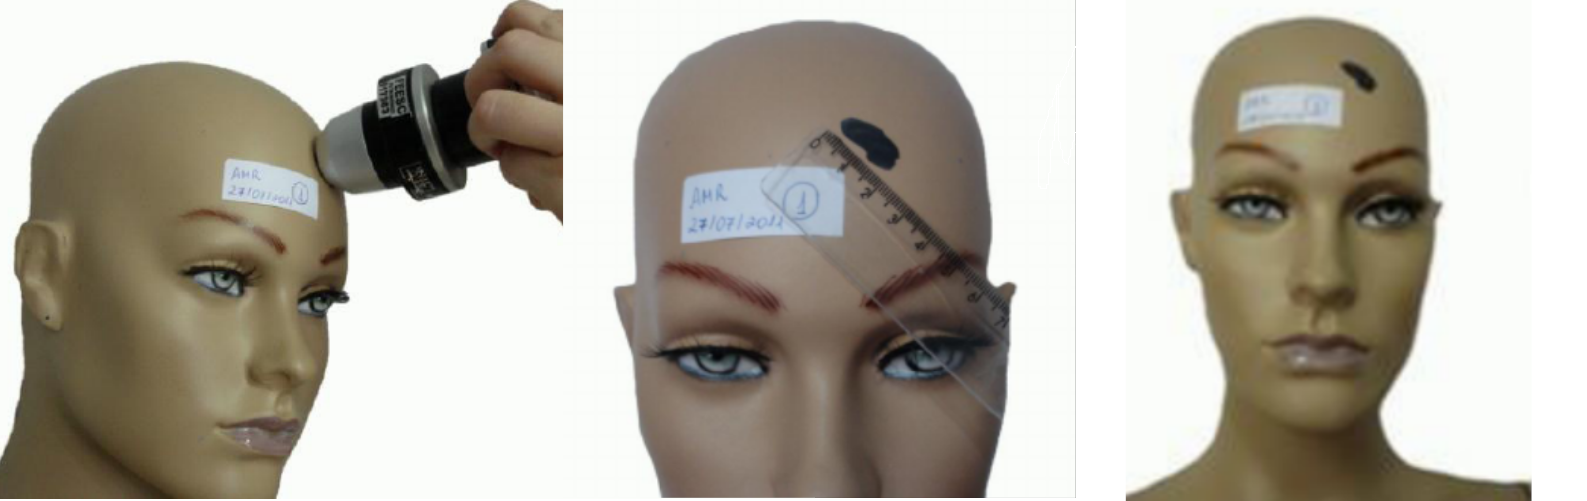
\includegraphics[width=1\columnwidth,keepaspectratio]{images/skin_lesion_exams.png}
    \caption{Exemplo de um exame de dermatoscopia, aproximação e panorâmica da cabeça, respectivamente. Fonte:
    \textcite{fotos_dermatologia}.}
    \label{fig:skin_lesion_exams}
\end{figure}

\subsection{\textit{Multimodal Large Language Models}}

\acp{mllm} são \acp{ia} baseadas em \acp{llm} que possuem a capacidade de interpretação de diferentes modalidades de
informação, como imagens, vídeos e áudios. O que torna esses modelos diferentes de \acp{llm}, que operam sobre
informações textuais. Esses modelos também podem ser capazes de gerar conteúdo \cite{mllm_survey_2023,
mllm_survey_2024}.

Segundo \textcite{mllm_survey_2024}, a estrutura de um \ac{mllm} pode ser dividida em cinco componentes, sendo eles o
codificador de modalidade, projetor de entrada, \ac{llm}, projetor de saída e o gerador de modalidade. No caso de
\acp{mllm} que possuem apenas saída de texto, somente os três primeiros componentes estão presentes, essa estrutura é
demonstrada na \autoref{fig:mllm_structure_encoder_only}.

\begin{figure}[ht]
    \centering
    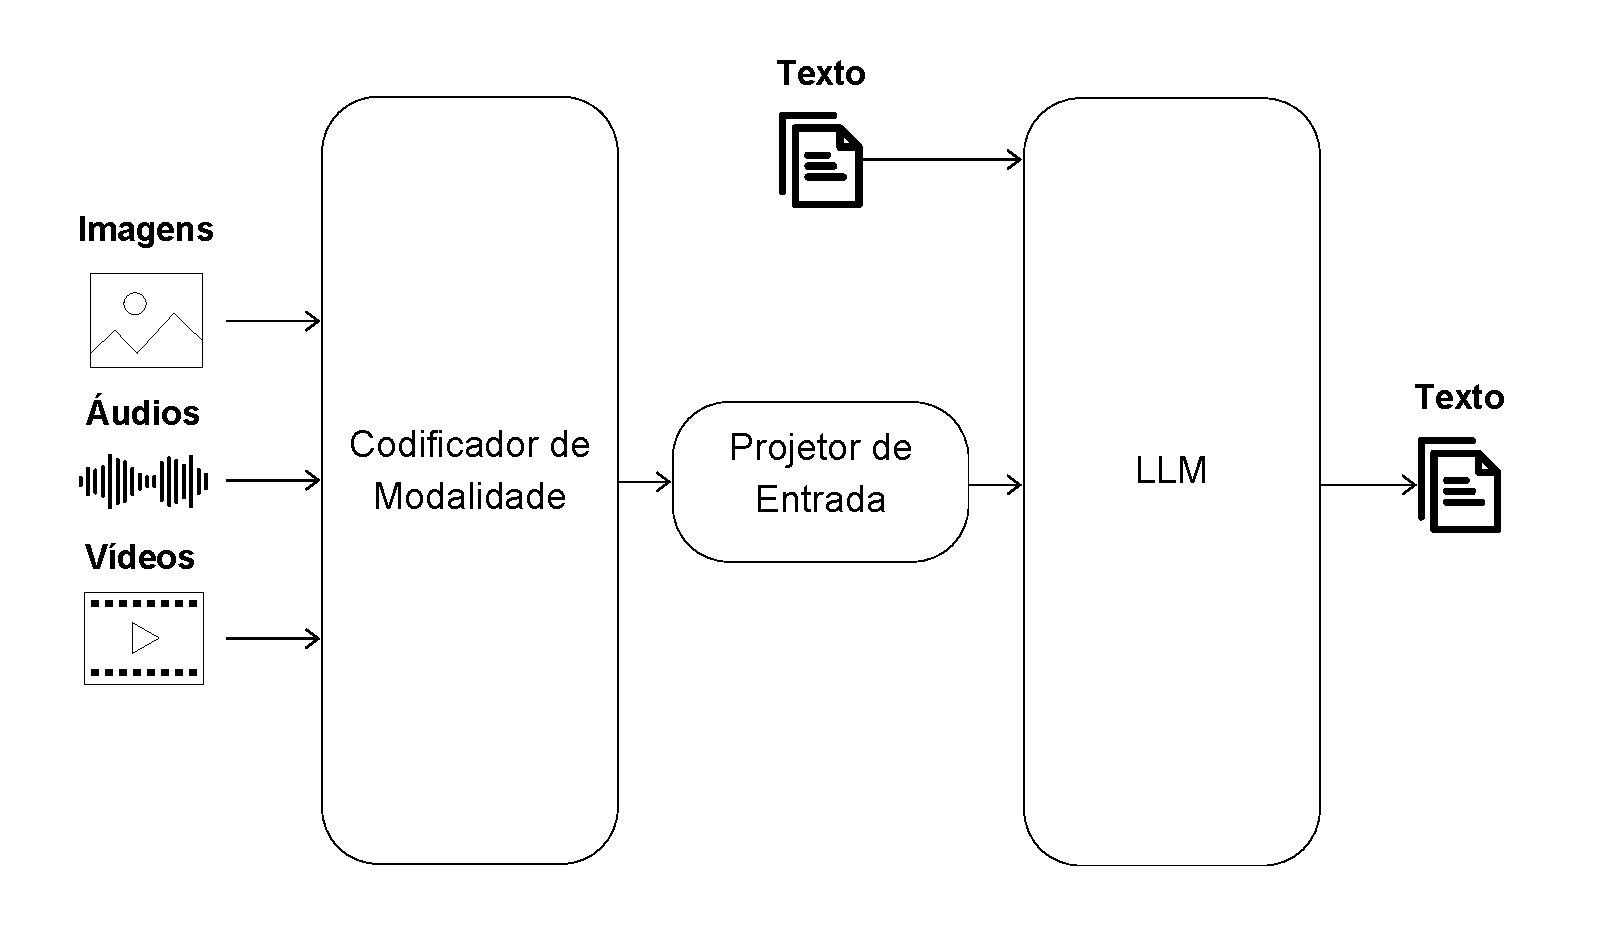
\includegraphics[width=0.7\columnwidth,keepaspectratio]{images/mllm_structure_encoder_only.pdf}
    \caption{Estrutura de um \ac{mllm} que realiza apenas a interpretação multimodal. Fonte: Autoria própria.}
    \label{fig:mllm_structure_encoder_only}
\end{figure}

\subsubsection{\textit{Large Language Models}}

\acp{llm} ou Grandes Modelos de Linguagem são modelos estatísticos pré-treinados baseados em transformadores que
possuem bilhões de parâmetros e conseguem processar e gerar textos em linguagem natural \cite{llm_survey_2024}.

Embora modelos de linguagem já sejam conceitos discutidos há várias décadas, a introdução da arquitetura de
transformadores no artigo \textit{Attention Is All You Need} de \textcite{transformer} define um marco no
desenvolvimento destes modelos, levando ao surgimento de \acp{llm}.

O funcionamento desta arquitetura pode ser explicada em diversas etapas. Inicialmente, antes do processamento no
transformador, o texto é dividido em partes menores, chamadas \textit{tokens}, no processo de tokenização. Geralmente,
essas partes se consistem de palavras ou partes de palavras. No transformador, os \textit{tokens} são então
representados em incorporações vetoriais, que se tratam de vetores em um espaço n-dimensional. Essas incorporações
passam pela codificação posicional, definindo as suas posições na sequência. Após a codificação posicional, o vetores
passam pelas camadas do transformador.

Na arquitetura original, o transformador possui um codificador e um decodificador, sendo que cada um deles é composto
por camadas diferentes. No codificador, cada camada é composta por duas subcamadas, sendo uma delas um mecanismo de
\textit{multi-head self-attention} e outra, uma rede \textit{feed-forward}. A saída de cada uma delas possui uma
conexão residual e uma etapa de normalização. O decodificador é similar ao codificador, mas suas camadas possuem uma
subcamada extra que aplica o mecanismo de \textit{multi-head self-attention} mascarado sobre a saída do codificador.
Além disso, a entrada do decodificador é deslocada em uma posição, de modo que uma nova incorporação possa ser prevista
e usada para gerar um \textit{token}. A \autoref{fig:transformer} mostra o transformador original.

\begin{figure}[ht]
    \centering
    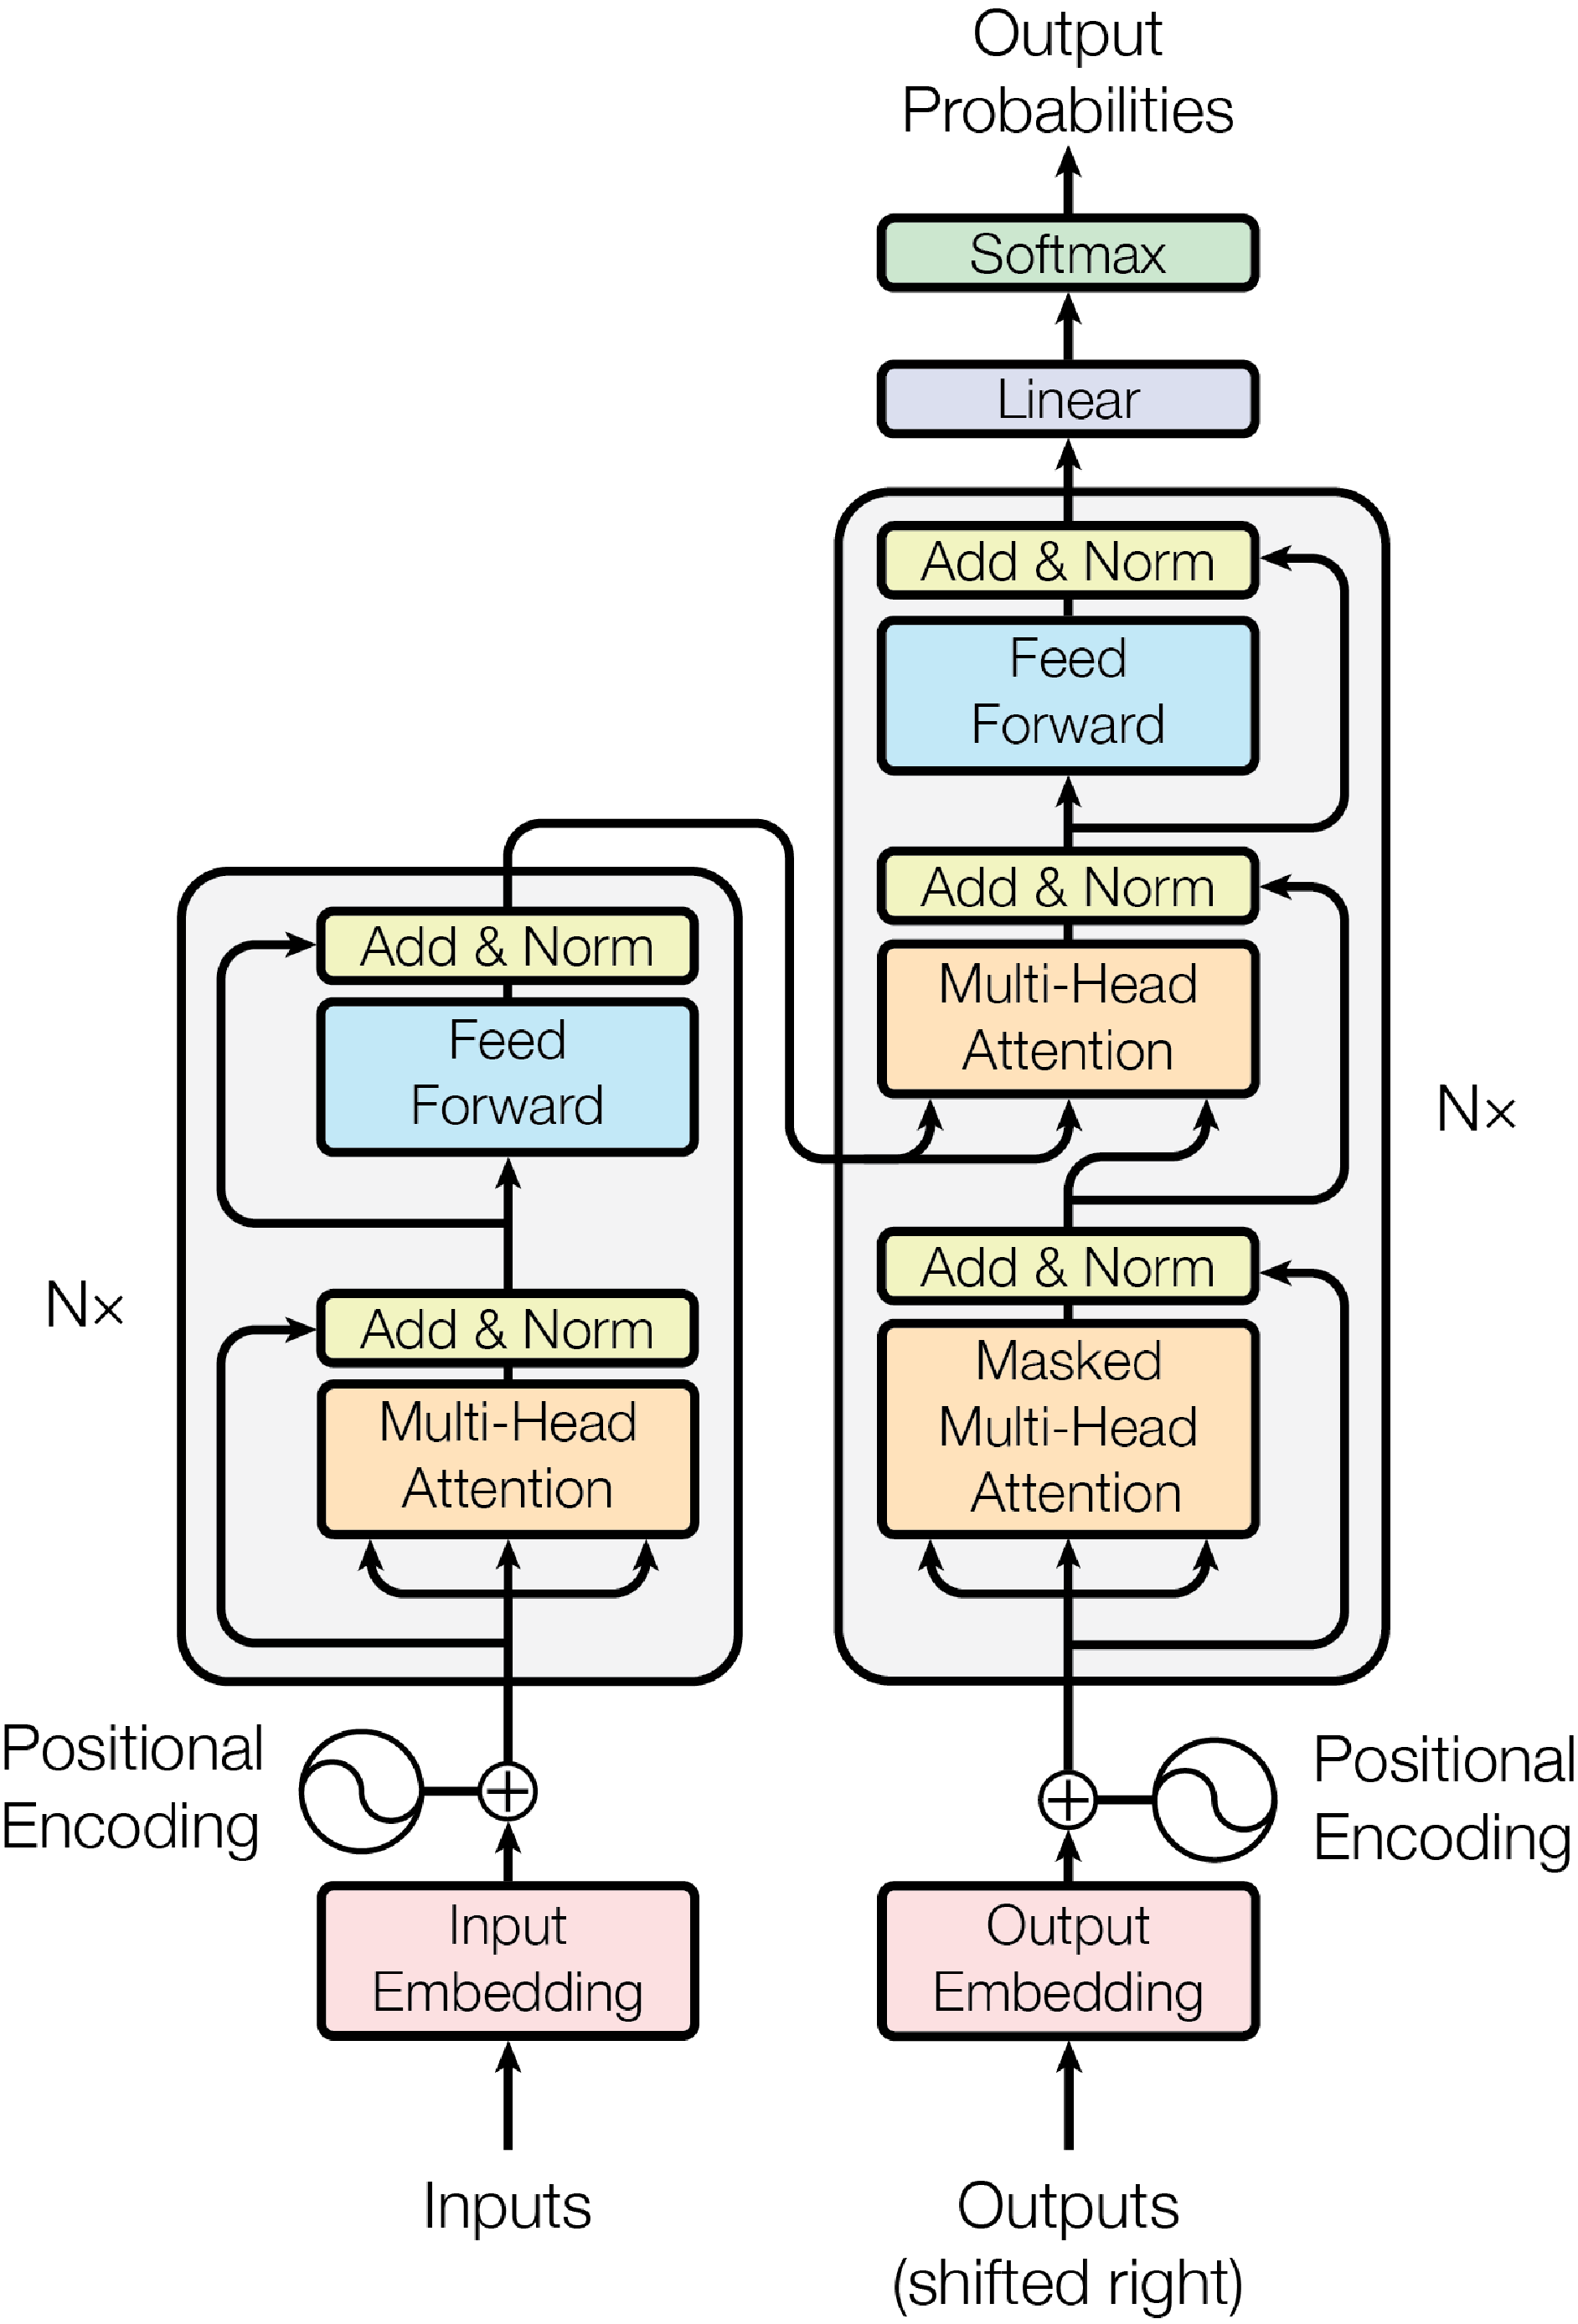
\includegraphics[width=0.4\columnwidth,keepaspectratio]{images/transformer.png}
    \label{fig:transformer}
    \caption{Arquitetura de um transformador. Fonte: \textcite{transformer}.}
\end{figure}

\subsubsection{Codificador de Modalidade}

Codificadores de modalidade são os componentes responsáveis pela extração das características mais relevantes dos dados
multimodais de entrada em incorporações vetoriais \cite{mllm_survey_2024}. Um exemplo de codificador de modalidade é o
codificador visual, do qual existem várias implementações. Os mais comuns usam \acp{vit} ou Transformadores Visuais nas
suas arquiteturas, mas também há codificadores baseados em convolução, como o \textit{Osprey} \cite{mllm_survey_2023}.

\acp{vit} são transformadores capazes de processar imagens introduzidos por \textcite{dosovitskiy2020image}.
A arquitetura original utiliza apenas codificadores e visa classificar imagens. O funcionamento desse tipo de
transformador é similar ao do modelo de \textcite{transformer}, com a tokenização de imagens em seções menores e a
representação dessas seções em incorporações vetoriais. A \autoref{fig:vision_transformer} demonstra a estrutura de
um transformador visual com os detalhes de sua implementação.

\begin{figure}[ht]
    \centering
    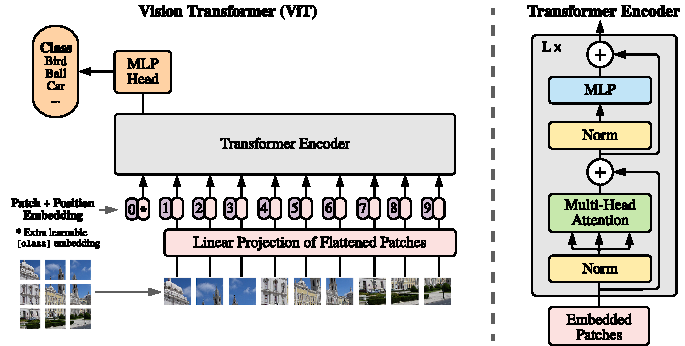
\includegraphics[width=0.8\columnwidth,keepaspectratio]{images/vision_transformer.pdf}
    \label{fig:vision_transformer}
    \caption{Transformador visual. Fonte: \textcite{dosovitskiy2020image}.}
\end{figure}

\subsubsection{Projetor de Entrada}

Esse componente faz o alinhamento entre o espaço de incorporações geradas pelo codificador e o espaço de incorporações
do \ac{llm}, podendo utilizar um \ac{mlp} ou um mecanismo de \textit{cross-attention}. A principal diferença de
\textit{cross-attention} para \textit{self-attention} nesse contexto está no uso dos vetores de \textit{key}
provenientes do codificador para o cálculo da atenção no transformador do \ac{llm} \cite{mllm_survey_2024}.

\subsubsection{Pré-treinamento e \textit{Fine-tuning}}

O pré-treinamento de um \ac{mllm} envolve um grande volume de dados e poder computacional, sendo particularmente
intensivo na parte de treinamento do \ac{llm} \cite{mllm_survey_2024}. Em geral, o modelo resultante deste processo é
generalista e não foca em nenhum domínio de conhecimento em particular.

O \textit{fine-tuning} é uma etapa de treinamento que pode ser realizada para melhorar o desempenho do modelo com
relação a dados específicos ou sobre um domínio de conhecimento. Técnicas de \textit{fine-tuning} eficientes, como as
baseadas em \ac{peft}, oferecem uma forma de adaptação de modelos com um custo computacional relativamente menor.
Dentre
várias técnicas, uma das mais populares é o treinamento com \ac{lora} \cite{llm_survey_2023}.

A técnica \ac{lora}, proposta por \textcite{hu2021lora}, consiste-se em explorar o \textit{rank} intrínseco, um
conceito baseado em dimensionalidade intrínseca, introduzindo matrizes treináveis menores de baixo \textit{rank} ao
\ac{mllm}, deixando as matrizes originais intactas durante o treinamento. Assim que treinadas, essas matrizes são
adicionadas às originais.

O \textit{rank} de uma matriz é o número de colunas ou linhas linearmente independentes que a matriz possui. Ele também
corresponde à dimensão do espaço vetorial gerado pelas colunas ou linhas. O \textit{rank} intrínseco se trata do menor
\textit{rank} que a matriz pode ter no treinamento sem haver uma grande perda de desempenho.

Assim, pode-se resumir que com base em uma matriz \begin{math}W_0\end{math} do modelo, tal que \begin{math}W_0 \in
    \mathbb{R}^{d \times k}\end{math}, é possível
representá-la em uma forma decomposta \begin{math}W_0 + \Delta W\end{math} em que \begin{math}\Delta W = BA\end{math},
tal que
\begin{math}B \in \mathbb{R}^{d \times r}\end{math} e \begin{math}A \in \mathbb{R}^{r \times k}\end{math}, sendo que
\begin{math}r \ll min(d, k)\end{math}. A matriz
\begin{math}W_0\end{math} é travada enquanto as matrizes \begin{math}A\end{math} e \begin{math}B\end{math} são
treináveis. A matriz \begin{math}A\end{math} é
inicializada com uma distribuição gaussiana aleatória e a \begin{math}B\end{math} é inicializada como zero. Na
\autoref{fig:lora} é apresentada uma representação visual
do \ac{lora} com a expressão \begin{math}h = W_0x + BAx\end{math}.

\begin{figure}[ht]
    \centering
    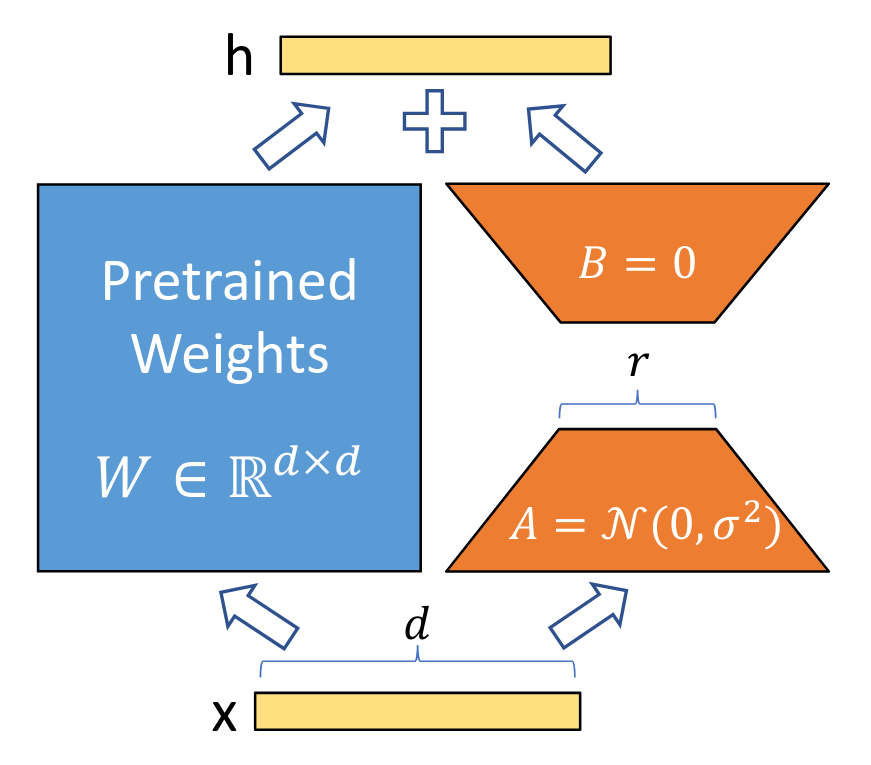
\includegraphics[width=0.35\columnwidth,keepaspectratio]{images/lora.png}
    \label{fig:lora}
    \caption{Representação do \ac{lora} com as matrizes \begin{math}W_0\end{math}, \begin{math}A\end{math} e
    \begin{math}B\end{math}. Fonte: \textcite{hu2021lora}.}
\end{figure}

É comum utilizar quantização para acelerar o \textit{fine-tuning}, onde se reduz precisão numérica durante o
treinamento. Uma técnica que utiliza este conceito é o \ac{qlora}, proposta por \textcite{qlora}. Nela, é usado o tipo
\ac{nf4} no armazenamento das matrizes pré-treinadas, sendo que os valores em \ac{nf4} são convertidos para \ac{bf16}
durante os cálculos. Além disso, também são usados otimizadores paginados e dupla quantização.

\subsection{LLaMA 3}

A família de modelos \ac{llama}-3 é composta por \acp{llm} e \acp{mllm} desenvolvidos pelos pesquisadores da
\textit{Meta AI}. Em particular, este trabalho focará no modelo multimodal \ac{llama}-3.2, que possui as variantes com
11 (\ac{llama}-3.2-11B) e 90 (\ac{llama}-3.2-90B) bilhões de parâmetros disponíveis \cite{dubey2024llama}.

O \ac{llm} base do \ac{llama}-3.2 utiliza um transformador decodificador que possui algumas diferenças em relação à
arquitetura original de \textcite{transformer}, as maiores diferenças já existem desde os modelos \ac{llama} e
\ac{llama}-2 e podem ser elencadas com base no trabalho de \textcite{touvron2023llama}:

\begin{itemize}
    \item \textbf{Pré-normalização}: As subcamadas são pré-normalizadas, em vez de serem normalizadas
          posteriormente;
    \item \textbf{Normalização}: A função de normalização usada é a \ac{rmsnorm};
    \item \textbf{Função de ativação}: Na subcamada de \textit{feed-forward}, a função de ativação é a \ac{swiglu},
          em vez de
          \ac{relu};
    \item \textbf{Codificação posicional}: A codificação posicional é feita com \ac{rope}, em vez da codificação
          absoluta;
    \item \textbf{\acs{gqa}}: \ac{gqa} é utilizado é com 8 cabeças de chave-valor para melhorar a velocidade de
          inferência e
          reduzir o tamanho dos \textit{caches} de chave-valor durante a decodificação;
    \item \textbf{Máscara de atenção}: Uma máscara é utilizada para impedir o relacionamento entre diferentes
          documentos de uma
          mesma entrada;
    \item \textbf{Vocabulário}: O vocabulário de \textit{tokens} usado possui 128 mil \textit{tokens}.
\end{itemize}

A \autoref{tab:llama3_architecture} apresenta alguns parâmetros das variantes do \ac{llm}.

\begin{table}[ht]
    \centering
    \begin{tabular}{l|ccc}
        \hline
                                               & 8B
                                               & 70B                                               & 450B
        \\ \hline
        Camadas do transformador               & 32
                                               & 80                                                & 126
        \\
        Dimensão das incorporações             & 4096
                                               & 8192                                              & 16384
        \\
        Dimensão da rede \textit{feed-forward} & 14336
                                               & 28672                                             & 53248
        \\
        \textit{fAttention heads}              & 32
                                               & 64                                                & 128
        \\
        \textit{fKey / Value heads}            & 8
                                               & 8                                                 & 8
        \\
        Taxa máxima de aprendizado             & \begin{math}3 \times 10^{-4}\end{math}
                                               & \begin{math}1.5 \times 10^{-4}\end{math}          & \begin{math}8
                                                                                                         \times

                                                                                                         10^{-5}\end{math} \\
        Função de ativação                     & \multicolumn{3}{c}{\ac{swiglu}}
        \\
        Tamanho do vocabulário                 & \multicolumn{3}{c}{128000}
        \\
        Codificação posicional                 & \multicolumn{3}{c}{\ac{rope}\begin{math}(\theta =
                                                                                 500000)\end{math}}
        \\ \hline
    \end{tabular}
    \label{tab:llama3_architecture}
    \caption{Características das variantes do \ac{llama}-3. Fonte: \textcite{dubey2024llama}.}
\end{table}

O codificador visual utilizado é baseado no transformador visual de \textcite{dosovitskiy2020image}, sendo usada a
variante \ac{vit}-H/14 com modificações extras, como a adição de extração de características multicamadas e de 8
camadas de \textit{gated self-attention}, deixando o codificador com um total de 850 milhões de parâmetros.

O projetor de entrada, referenciado como adaptador de visão no trabalho de \textcite{dubey2024llama}, se baseia em
\textit{cross-attention} entre as camadas de codificação do codificador visual e as camadas de decodificação do
\ac{llm}. Mais especificamente, é aplicada uma camada de \textit{cross-attention} a cada quarta camada do \ac{llm}.
Essas camadas também utilizam \ac{gqa} para melhorar o desempenho.

Além de imagens, o \ac{llama}-3.2 também pode operar com vídeos e áudios. A \autoref{fig:llama} apresenta a arquitetura
multimodal do modelo.

\clearpage

\begin{figure}[ht]
    \centering
    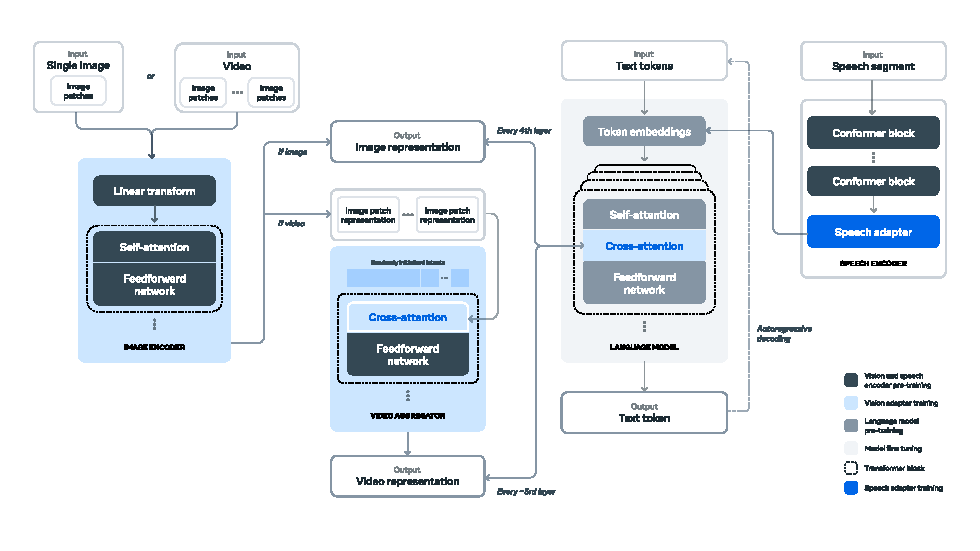
\includegraphics[width=1.0\columnwidth,keepaspectratio]{images/llama.pdf}
    \label{fig:llama}
    \caption{Arquitetura multimodal de imagem e vídeo do \ac{llama}-3.2. Fonte: \textcite{dubey2024llama}.}
\end{figure}
